\chapter{Preliminares}
En este capítulo, se presentarán los conceptos básicos sobre diferenciación compleja y la teoría de las funciones analíticas que se utilizarán a lo largo de este trabajo. También se establecerá la notación y otros conceptos relevantes.
\section{Funciones complejo diferenciables} \label{sec:Fcd}\index{Funciones complejo diferenciables}
Esta sección está dedicada a presentar el concepto de funciones diferenciables complejas. Sin embargo, antes de ello, recordaremos los conceptos de número complejo, valor absoluto y argumento.\\
Los números complejos, denotados por $\C$, son una extensión de los números reales. Se forman al dotar al conjunto de pares ordenados $(a, b), con a, b \in \R$ con las siguientes operaciones:

\begin{itemize}
	\item [1)] $(a, b) + (c, d) = (a + c, b + d)$,
	\item [2)] $(a, b)\cdot(c, d) = (ac - bd, ad + bc).$
\end{itemize}
Con estas operaciones tenemos que $(\C,+,\cdot)$ es un campo.\\
\noindent Dado $z=(a,b)\in \C$, normalmente escribiremos $$z=a+bi,$$
donde $i=\sqrt{-1}$. Diremos que $a$ y $b$ son las partes real e imaginaria de $z$ respectivamente y se escribirá
$$a=\operatorname{Re}(z)\atop b=\operatorname{Im}(z)$$
\begin{defi}
	Sean $z=a+ib\in\C$, y $O=(0,0)$, $P=(a,b)$ los puntos en el plano complejo para el origen y $z$ respectivamente, además sea $\vec{OP}$ el vector que une al origen con $z$
	\begin{itemize}
		\item [1)] Se define el conjugado de $z$ como $$\overline{z}=a-ib.$$
		\item [2)] Se define el valor absoluto (a veces llamado módulo o norma) de $z$ como $$|z|=\sqrt{a^2+b^2}$$
		\item [3)] Se define el argumento de $z$ como el ángulo que se forma entre el eje real positivo  y el vector $\vec{OP}$ y lo denotaremos por $\operatorname{Arg}(z)$
	\end{itemize}
\end{defi}
\noindent Entre los valores del argumento del número $z\neq 0$, existe uno, y sólo uno, comprendido entre $-\pi$ y $\pi$. Este se denomina valor principal del argumento y se denota por $\operatorname{arg}(z)$. Así, pues, $$-\pi<\operatorname{arg}(z)<\pi$$
y $$\operatorname{Arg}(z)=\operatorname{arg}+2n\pi,$$
donde $n$ recorre todos los números enteros.  
\begin{defi}
	Sea $\Omega\subset \C$ un conjunto abierto y sea $a \in \Omega$. Sea $f:\Omega\rightarrow\C$, entonces $f$ es complejo diferenciable en $a$ si el siguiente límite existe
	$$\lim_{h\rightarrow 0} \dfrac{f(a+h)-f(a)}{h}=\lim_{z\rightarrow a}\dfrac{f(z)-f(a)}{z-a}.$$
	El valor de este límite se denota por $f'(a)$ y se llama la derivada de $f$ en $a$. Si $f$ es diferenciable en cada punto de $\Omega$, diremos que $f$ es complejo diferenciable en $\Omega$. Además, si $f'$ es continua en $\Omega$, entonces $f$ se llama continuamente diferenciable en $\C$. Y si $f$ tiene diferenciales de todos los órdenes, se llama infinitamente diferenciable en $\C$.
\end{defi}
El siguiente teorema es una es una equivalencia de la definición anterior. La prueba se puede consultar en \cite{silverman}, específicamente vea el Teorema 3.1 de dicha referencia.

\begin{teor}\label{teodif}
	Sean $\Omega\subset \C$ abierto, $a\in\C$ y $f:\Omega\rightarrow\C$. Entonces $f$ es complejo diferenciable en $a$ si y sólo si puede escribirse de la siguiente forma:
	\begin{equation}
		f(z)-f(a)=A(z-a)+(z-a)\varepsilon(z,a),
	\end{equation}
	 en donde $\varepsilon(z,a)\rightarrow 0$ cuando $z\rightarrow a$ y $A$ es una constante independiente de $(z-a)$ y $\varepsilon$.
	
\end{teor}

Si es $f$ una función complejo diferenciable en $a$, entonces por el Teorema \ref{teodif}, $f$ puede escribirse 
$$f(z)-f(a)=A(z-a)+(z-a)\varepsilon(z,a),$$
donde $\varepsilon(z,a)\rightarrow 0$ cuando $z\rightarrow a$ y $A$ es una constante. Si $z\rightarrow a$, entonces
\[
\begin{array}{ccl}
	\ds\lim_{z\rightarrow a}f(z)&=&\ds\lim_{z\rightarrow a}[f(a)+A(z-a)+(z-a)\varepsilon(z,a)]\\
	&=&f(a)+A\ds\lim_{z\rightarrow a}(z-a)+\ds\lim_{z\rightarrow a}[(z-a)\varepsilon(z,a)]\\
	&=&f(a).
\end{array}
\]
Por lo tanto, $f$ es continua en $a$. En resumen se tiene la siguiente proposición.
\begin{prop}
	Sea $\Omega\subset \C$ un conjunto abierto y sea $a \in \Omega$. Sea $f:\Omega\rightarrow\C$, si $f$ es complejo diferenciable en $a$, entonces es continua en $a$.
\end{prop}
\begin{defi}
	Una función $f:\Omega\rightarrow\C$ es analítica si $f$ es complejo diferenciable en todo punto de  $\Omega$. Si $f(z)$ es analítica en un vecindad de $a\in \Omega$, diremos que $f(z)$ es analítica en $a$.
\end{defi}

\begin{prop}
	Sea $\Omega\subset \C$ un conjunto abierto y sea $a \in \Omega$. Sean $f,g:\Omega\rightarrow\C$ complejo diferenciables en $\Omega$. Entonces 
	\begin{itemize}
		\item [(1)] $(f+g)(z)=f(z)+g(z)$ es complejo diferenciable en $\Omega$.
		\item [(2)] $(fg)(z)=f(z)g(z)$ es complejo diferenciable en $\Omega$.
		\item [(3)] Si $g(z)\neq 0$ para $z\in\Omega$, entonces $\dfrac{f}{g}(z) = \dfrac{f(z)}{g(z)}$ es complejo diferenciable en $\Omega$.
	\end{itemize} 
\end{prop}
El lector interesado puede consultar la Proposición 1.5.3 de \cite{marsden}. 
\begin{teor}[Regla de la cadena]
	Sean $f$ y $g$ funciones complejo diferenciables en $\Omega$ y $\Omega_{1}$ respectivamente y suponga que $f(\Omega)\subset\Omega_{1}$. Entonces $g\circ f$ es complejo diferenciable sobre $\Omega$ y 
	$$(g\circ f)'(z)=g'(f(z))f'(z).$$
	La demostración de este teorema no es difícil, en esencia es usar el Teorema \ref{teodif}, sugerimos al lector ver la Proposición 2.4 de \cite{Conway}.


\end{teor}
\section{Ecuaciones de Cauchy-Riemann} \label{sec:Cauchy-Riemann}

Sea $f:\Omega\rightarrow\C$ una función complejo diferenciable y sea $z=x+iy\in \Omega$. Entonces podemos escribir
$$f(z)=f(x+iy)=u(x,y)+iv(x,y),$$
donde $u(x,y)=\mathrm{Re } f(x+iy)$ y $v(x,y)=\mathrm{Im } f(x+iy)$. Ahora evaluaremos el límite 
$$f'(z)=\lim_{h\rightarrow 0}\dfrac{f(z+h)-f(z)}{h},$$
de dos diferentes maneras.\\
Primero evaluaremos cuando $h\rightarrow 0$ y $h\in \R\setminus\{0\}$. En este caso  se tiene que
\[
\begin{array}{ccl}
	\dfrac{f(z+h)-f(z)}{h}&=&\dfrac{f(x+h+iy)-f(x+iy)}{h}\\
	&=&\dfrac{u(x+h,y)-u(x,y)}{h}+i\dfrac{v(x+h,y)-v(x,y)}{h}.
\end{array}
\]

Luego, valuando el límite $h\rightarrow 0$ se obtiene
\begin{equation}\label{ec2}
	f'(z)=\dfrac{\partial u}{\partial x}(x,y)+i\dfrac{\partial v}{\partial x}(x,y).
\end{equation}

Ahora evaluemos cuando $h\rightarrow 0$ y $h$ es un complejo puro distinto de cero. 
\[
\begin{array}{ccl}
	\dfrac{f(z+ih)-f(z)}{ih}&=&-i\dfrac{u(x,y+h)-u(x,y)}{h}+\dfrac{v(x,y+h)-v(x,y)}{h},
\end{array}
\]
tomando el límite cuando $h\rightarrow 0$, obtenemos  
\begin{equation}\label{ec3}
	f'(z)=-i\dfrac{\partial u}{\partial{y}}(x,y)+\dfrac{\partial v}{\partial y}(x,y).
\end{equation}
Finalmente, combinando de las ecuaciones (\ref{ec2}) y (\ref{ec3}), obtenemos el siguiente par de ecuaciones 
\begin{equation}
	\dfrac{\partial u}{\partial x} = \dfrac{\partial v}{\partial y}\hspace{0.5 cm} \mbox{ y } \hspace{0.5 cm} \dfrac{\partial u}{\partial y} =- \dfrac{\partial v}{\partial x},
\end{equation}
las cuales se conocen como ecuaciones de \textbf{Cauchy-Riemann}, lo anterior prueba el siguiente teorema.

\begin{teor}\label{teo3}
		Sean $\Omega\subset \C$ un conjunto abierto y $z_{0}=(x_{0},y_{0}) \in \Omega$. Si $f:\Omega\rightarrow\C$ es una función complejo diferenciable  en $z_{0}$, entonces
		\[
			\begin{array}{ccl}
				\dfrac{\partial u}{\partial x} = \dfrac{\partial v}{\partial y} &\mbox{ y } & \dfrac{\partial u}{\partial y} =-\dfrac{\partial v}{\partial x},
			\end{array}
		\]
		donde $f(x,y)=(u(x,y),v(x,y))$.
\end{teor}


\begin{teor}[Ecuaciones de Cauchy-Riemann]\label{TECR}
	Sea $$f(z)=u(x,y)+iv(x,y),$$ una función definida en un dominio $\Omega$. Entonces una
	condición necesaria y suficiente para que $f (z)$ sea complejo diferenciable en el punto
	$z_0 = x_0 + iy_0 \in \Omega$, es que las funciones $u(x, y)$ y $v(x, y)$ sean real diferenciables en el
	punto $z_0=(x_0, y_0)$ y que satisfagan las ecuaciones de Cauchy-Riemann. Si estas condiciones se cumplen, $f'(z_0)$, puede representarse en cualquiera de las siguientes formas:
	\begin{equation}
		f'(z_0)=\dfrac{\partial u}{\partial x}+i\dfrac{\partial v}{\partial x}=\dfrac{\partial v}{\partial y}-i\dfrac{\partial u}{\partial y}=\dfrac{\partial u}{\partial x}-i\dfrac{\partial u}{\partial y}=\dfrac{\partial v}{\partial y}+i\dfrac{\partial v}{\partial x},
	\end{equation}
	 en donde las parciales son evaluadas en $(x_0, y_0)$.\\
	La demostración de este teorema se puede consultar en \cite{silverman}, vea el Teorema 3.2.
\end{teor}

En ocasiones, se usa el término función \textbf{holomorfa} o \textbf{regular} en lugar de función analítica. Si  $\Omega\subset \C$ es un conjunto abierto, utilizaremos la siguiente notación:
$$\mathcal{H}(\Omega)=\{f:\Omega\rightarrow \C \mid f \mbox{ es holomorfa en } \Omega\},$$
para referirnos al conjunto de funciones holomorfas en $\Omega$.\\
Una función holomorfa en todo $\C$   es llamada una función \textbf{entera}.
\begin{Ejem}
	Consideremos la función $f(z)=|z|^{2}$, trataremos primero esta función como una función de $\R^2\rightarrow\R$, es decir, $z=(x,y)\in\R^2$, tenemos 
	$$f(z)=f(x,y)=|(x,y)|^2=\left(\sqrt{x^{2}+y^{2}}\right)^2=x^2+y^2.$$
	Sea $a=(a_1,a_2)\in\R^2$ un elemento arbitrario, entonces 
	\[
	\begin{array}{ccl}
		\dfrac{f(x,y)-f(a_1,a_2)-2a_1(x-a_1)-2a_2(x-a_2)}{\sqrt{(x-a_1)^2+(y-a_2)^2}}&=&\dfrac{x^2+y^2-a_1^2-a_2^2}{\sqrt{(x-a_1)^2+(y-a_2)^2}}+\\
		&&+\dfrac{-2a_1(x-a_1)-2a_2(x-a_2)}{\sqrt{(x-a_1)^2+(y-a_2)^2}}\\
		&=&\dfrac{(x-a_1)^2+(y-a_2)^2}{\sqrt{(x-a_1)^2+(y-a_2)^2}}\\
		&=&\sqrt{(x-a_1)^2+(y-a_2)^2}.
	\end{array}
	\]
	Al tomar el límite cuando $(x,y)\rightarrow(a_1,a_2)$, se tiene que $f(x,y)$ es real diferenciable en $a=(a_1,a_2)$ y dado que $a$ fue arbitrario $f(x,y)$ es diferenciable en $\R^2$.\\
	Ahora, consideremos  $f(z)=|z|^{2}$ como un mapeo de $\C\rightarrow\C$.
	Tenemos que si $z=x+iy$, entonces 
	$$f(z)=|z|^2=|x+iy|^2=x^2+y^2,$$
	luego, si $u(x,y)=\mbox{Re }f(z)$ y $v(x,y)=\mbox{Im }f(z)$, entonces $u(x,y)=x^2+y^2$ y $v(x,y)=0$.\\ 
	Además
	\[
	\begin{array}{ccl}
		\dfrac{\partial u}{\partial x}&=&2x,\\
		\dfrac{\partial v}{\partial y}&=&0,\\
		\dfrac{\partial u}{\partial y}&=&2y,\\
		\dfrac{\partial v}{\partial x}&=&0.
	\end{array}
	\]
	Notemos que las ecuaciones de Cauchy-Riemann se cumplen solo si $(x,y)=(0,0)$, es decir, $f(z)$ es complejo diferenciable solo en $(0,0)$. Por otro lado, si $z_0\in \C\setminus\{0\}$, entonces 
	\[
	\begin{array}{ccl}
		\displaystyle	\lim_{z\rightarrow z_0}\dfrac{|z|^2-|z_0|^2}{z-z_0}&=&\displaystyle\lim_{z\rightarrow z_0}\dfrac{|z|-|z_0|}{z-z_0}(|z|+|z_0|),
	\end{array}
	\]
	luego, si $z$ tiende a $z_0$ a lo largo del rayo $\{\alpha z_0\mid \alpha\in (1,\infty)\}$, entonces 
	el límite anterior es $2\overline{z_0}\neq 0$. Por tanto, no existe un abierto $\Omega\subset \C$ en el que $f(z)$ sea holomorfa.\endproof
\end{Ejem}
El ejemplo anterior ilustra una función que puede ser diferenciable en términos reales, pero no en términos complejos. Esto resalta la distinción entre la diferenciabilidad en el contexto de los números reales y los números complejos.
\begin{teor}[De Identidad para Funciones Analíticas]\label{TIFA}
	Si dos funciones analíticas reales $f(z)$ y $g(z)$, definidas en un dominio $\Omega$,
	coinciden en un conjunto $E \subset \Omega$ con punto límite $z_0 \in \Omega$, entonces $f(z)$ y $g(z)$ coinciden en todo el dominio $\Omega$.\\
	Para ver la demostración de este teorema, le sugerimos revisar el Teorema 10.8 de \cite{silverman}.
\end{teor} 
\begin{defi}
	Se dice que $a\in \C$ es una \textbf{singularidad aislada} de $f$ si $f$ es analítica en $D(a,r)\setminus\{a\}$ y no lo es en $D(a,r)$ para algún $r>0$.\\Por otra parte, diremos que $a$ es una \textbf{singularidad removible} de $f$ si existe $g$ analítica en $D(a,r)$ tal que $f=g$ en $D(a,r)\setminus\{a\}$.\\Una singularidad aislada a de $f$ es llamada \textbf{polo} si $\ds\lim_{z\rightarrow a}|f(z)|=\infty$; es decir, para todo $M>0$ existe $\delta>0$ tal que si $0<|z-a|<\delta$ entonces $|f(z)|>M$. Una singularidad que no es un polo ni una singularidad removible se llamará
	\textbf{singularidad esencial}.\\Sea $a$ un polo de $f$, el mínimo número natural $m$ tal que $f(z)(z-a)^m$ tiene una singularidad removible en $a$ será llamado el \textbf{orden del polo} en $a$.
\end{defi}
Acabamos de introducir los términos de singularidad aislada, removible, esencial y polo.  A partir de \textbf{Mathematica 12.0}, se incluyeron dos funciones que  nos permiten graficar mapeos complejos:  \textbf{ComplexPlot} y \textbf{ComplexPlot3D}. A continuación explicamos brevemente estas funciones.\\
\textbf{ComplexPlot} utiliza una función de color cíclica sobre Arg[$f$] para identificar características como ceros, polos y singularidades esenciales. La función de color va de $-\pi$ a $\pi$ en sentido contrario a las agujas del reloj alrededor de los ceros, en el sentido de las agujas del reloj alrededor de los polos, y ciclos infinitos cerca de las singularidades esenciales. Por convención los colores van en el siguiente orden: rojo, verde, azul, siguiendo un patrón RGB, el argumento es el que determina el color.
\begin{figure}[h!]
	\centering
	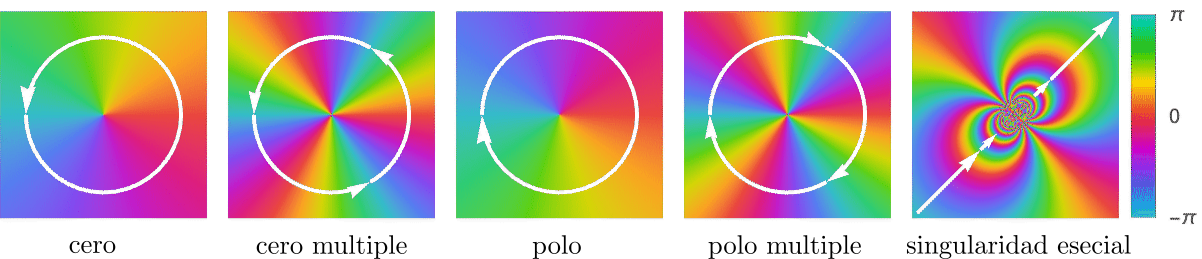
\includegraphics[width=0.75\linewidth]{img/plotco}
	\caption{Ejemplo gráfico del comportamiento de los ceros, polos y singularidades cuando se usa la función ComplexPlot3D}
	\label{fig:plotco}
\end{figure}
\\Y la forma de usar esta función es \textbf{ComplexPlot[$f$,$\{z,z_{min},z_{max}\}$]}, cabe aclarar que esta función genera un grafico de $\mathbf{\operatorname{Arg}[f]}$ sobre el rectángulo en el plano complejo con esquinas $z_{min}$ y $z_{max}$, además que,  la intensidad de los colores esta determinada por el valor absoluto (módulo) de $f$, es decir,  $\mathbf{\operatorname{Abs}[f]}$.\\
Por otro lado, recordemos que una función de variable compleja, $f(z)=w$ necesita de cuatro dimensiones para representarla gráficamente, pero visualizarla no es posible para los seres humanos. Sin embargo, podemos usar una proyección de esta superficie en cuatro dimensiones para dibujar la grafica en tres dimensiones. Para este fin, usaremos la función  \textbf{ComplexPlot3D}. Esta función al igual que ComplexPlot, determina la intensidad del color por el módulo y es el argumento el que determina el color. Esta función toma por parámetros la función $f$ y las esquinas de un rectángulo en el plano complejo cuyas esquinas son $z_{min}$ y $z_{max}$. \\

\noindent Al lector interesado le sugerimos revisar \cite{Domain_coloring}, allí encontrará una explicación más detallada, sin llegar a ser teórica, acerca de la visualización de funciones complejas usando colores.\\

En la versión 12.1 de \textbf{Mathematica} se introdujo la función \textbf{ComplexContourPlot}, la cual se utiliza para  visualizar gráficamente funciones complejas en el plano complejo. Esta función representa líneas de nivel de la parte real e imaginaria de la función compleja en el plano complejo, proporcionando una manera efectiva de ver cómo la función afecta la deformación del plano. En la practica, generalmente se usaran funciones como Re, Im, Abs y Arg para extraer las partes reales, imaginarias, el módulo y el argumento respectivamente para obtener la representación.


\begin{defi}
	Sean $f\colon \Omega\to\C$ una función, $a$ un punto interior de $\Omega$ y $r>0$ tal que la cerradura del disco $D(a,r)$ está contenida en $\Omega$. Definimos $A_{f,a,r}\colon[0,2\pi)\to\R$,
	\[
	A_{f,a,r}(\theta) = \operatorname{Arg}(f(a+re^{i\alpha})).
	\]
\end{defi}

\begin{teor}
	Sea $f\colon \Omega\to\C$ una función holomorfa
	y sea $a$ un punto interior del dominio $\Omega$.
	Supongamos que $a$ es un cero de $f$ de orden $m$.
	Entonces, existe $R>0$ tal que para cada $r$ que satisface $0<r<R$,
	la función $A_{f,a,r}$ recorre $m$ veces los valores de $-\pi$ a $\pi$.
\end{teor}

\noindent Usando la función \textbf{Plot3D} de \textbf{Mathematica} podemos visualizar el mapeo como una función de $\R^2 \rightarrow \R$ como sigue
\begin{mmaCell}[functionlocal=y]{Code}
	  Plot3D[x^2 + y^2, {x, -10, 10}, {y, -10, 10}]
\end{mmaCell}

\begin{mmaCell}[moregraphics={moreig={scale=.4}}]{Output}
	\mmaFrac{ \mmaGraphics{1.png}}{}
\end{mmaCell}

Tratando esta función como mapeo de $\C$ a $\C$ y utilizando las funciones \textbf{ComplexPlot} y \textbf{ComplexPlot3D}

\begin{mmaCell}[functionlocal=y]{Code}
	 ComplexPlot[Abs[z]^2, {z, -2 - 2 I, 2 + 2 I}]
\end{mmaCell}

\begin{mmaCell}[moregraphics={moreig={scale=.35}}]{Output}
	\mmaFrac{ \mmaGraphics{1_1.png}}{}
\end{mmaCell}

\begin{mmaCell}{Input}
  ComplexPlot3D[Abs[z]^2, \{z, -2 - 2 I, 2 + 2 I\},\\ColorFunction -> "CyclicLogAbs"]
\end{mmaCell}

\begin{mmaCell}[moregraphics={moreig={scale=.4}}]{Output}
	\mmaFrac{ \mmaGraphics{1_2.png}}{}
\end{mmaCell}
Como podemos ver, al ser $|z|^2$ una función que tiene por codominio los reales, \textbf{Mathematica} la interpreta como un función real al momento de graficarla, y esto último lo podemos comprobar cuando usamos \textbf{ComplexContourPlot}, donde observamos como solo se grafican las curvas de nivel de la componente real sin embargo no se grafica la componente compleja, incluso si le indicamos a Mathematica que la grafique, como lo hicimos en el código que sigue, esta grafica no se dibujará. Este código puede ser redundante pero solo es para fines ilustrativos, siguiendo las buenas practicas y quitando fragmentos de codigo innecesario solo basta quitar \textbf{Im[Abs[z]*Abs[z]}.
\begin{mmaCell}{Input}
	 ComplexContourPlot[\{Re[Abs[z]*Abs[z]], Im[Abs[z]*Abs[z]]\},\\\{z, 20\}, PlotLegends -> "Expressions"]
\end{mmaCell}

\begin{mmaCell}[moregraphics={moreig={scale=.35}}]{Output}
	\mmaFrac{ \mmaGraphics{contorno1.png}}{}
\end{mmaCell}


\begin{Ejem}
	Sea $f(z)=z=x+iy$, entonces $u(x,y)=x$ y $v(x,y)=y$. Tenemos
	$$u_x=1=v_y,$$
	$$u_y=0=-v_x.$$
	Como lo anterior se cumple para cualquier $z\in \C$, entonces $f(z)=z$ es complejo diferenciable en todo $\C$.\\
	Usando \textbf{Mathematica}
	\begin{mmaCell}{Input}
		ComplexPlot[z, \{z, -2 - 2 I, 2 + 2 I\}]
	\end{mmaCell}

	\begin{mmaCell}{Input}
		ComplexPlot3D[z, \{z, -2 - 2 I, 2 + 2 I\}]
	\end{mmaCell}

	\begin{mmaCell}{Input}
		ComplexContourPlot[\{Re[z], Im[z]\}, \{z, 2\},\\PlotLegends -> "Expressions"]
	\end{mmaCell}
El código anterior genera las imágenes mostradas en la figura \ref{fig:ej_4}.\\	
	\begin{figure}[htbp!]
		\centering
		\begin{subfigure}{0.25\textwidth}
			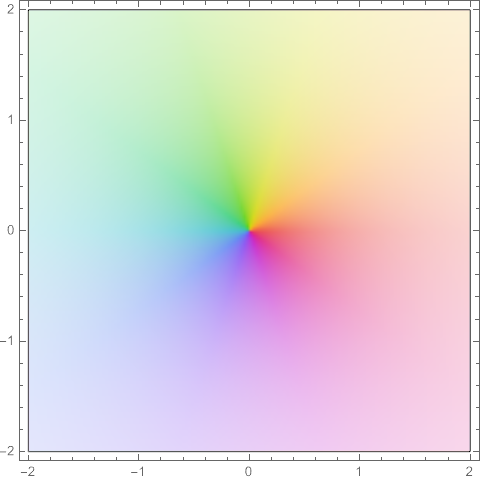
\includegraphics[width=\linewidth]{4_1.png}
			\caption{ComplexPlot.}
			\label{fig:ej_4_1}
		\end{subfigure}
		\begin{subfigure}{0.25\textwidth}
			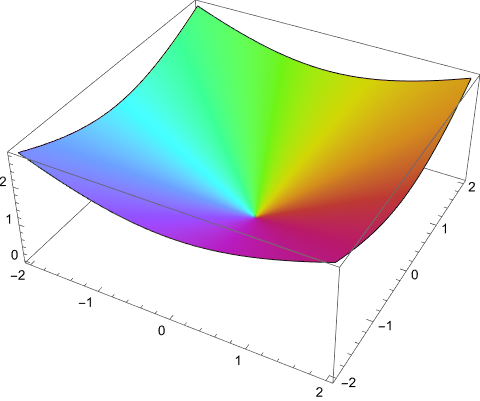
\includegraphics[width=\linewidth]{4_2.png}
			\caption{ComplexPlot3D.}
			\label{fig:ej_4_2}
		\end{subfigure}
		\begin{subfigure}{0.25\textwidth}
			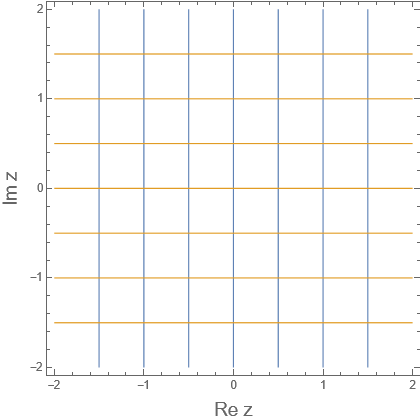
\includegraphics[width=\linewidth]{4_3.png}
			\caption{ComplexContourPlot.}
			\label{fig:ej_4_3}
		\end{subfigure}
		\caption{Diferentes representaciones graficas de la función $f(z)=z$}
		\label{fig:ej_4}
	\end{figure}

\noindent En la figuras \ref{fig:ej_4_1} y \ref{fig:ej_4_2} podemos ver que la función $f(z)=z$ tiene un cero en $z=0$, mientras que en la figura \ref{fig:ej_4_3} vemos que la función identidad no deforma el plano.
\end{Ejem} 


\begin{Ejem}
	Sea $f(z)=\overline{z}=x-iy$, entonces $u(x,y)=x$ y $v(x,y)=-y$. Tenemos
	$$u_x=1,$$
	$$v_y=-1,$$
   entonces $f(z)=\bar{z}$ es no diferenciable en $\C$.\\
	Usando \textbf{Mathematica}
	\begin{mmaCell}{Input}
		ComplexPlot[Conjugate[z], \{z, -2 - 2 I, 2 + 2 I\}]
	\end{mmaCell}
	
	\begin{mmaCell}{Input}
		ComplexPlot3D[Conjugate[z], \{z, -2 - 2 I, 2 + 2 I\}]
	\end{mmaCell}
	
	\begin{mmaCell}{Input}
		ComplexContourPlot[\{Re[Conjugate[z]], Im[Conjugate[z]]\}, \\\{z, 2\},PlotLegends -> "Expressions"]
	\end{mmaCell}
	Obtenemos las figuras mostradas en la figura \ref{fig:ej_4}.\\	
	\begin{figure}[htbp!]
		\centering
		\begin{subfigure}{0.25\textwidth}
			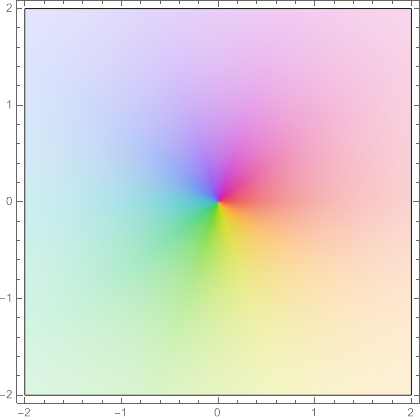
\includegraphics[width=\linewidth]{5_1.png}
			\caption{ComplexPlot.}
			\label{fig:ej_5_1}
		\end{subfigure}
		\begin{subfigure}{0.25\textwidth}
			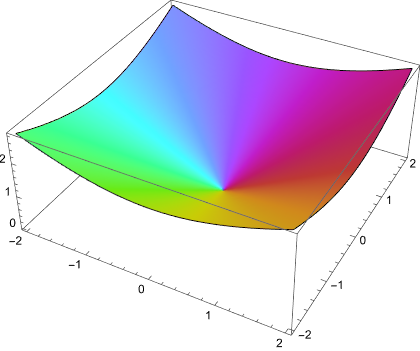
\includegraphics[width=\linewidth]{5_2.png}
			\caption{ComplexPlot3D.}
			\label{fig:ej_5_2}
		\end{subfigure}
		\begin{subfigure}{0.25\textwidth}
			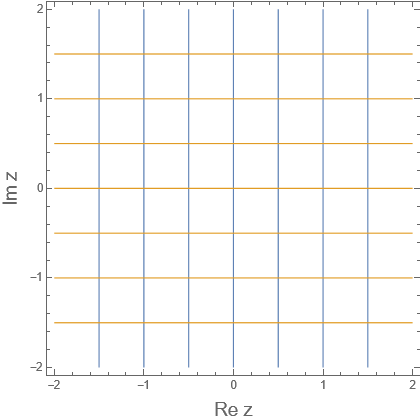
\includegraphics[width=\linewidth]{5_3.png}
			\caption{ComplexContourPlot.}
			\label{fig:ej_5_3}
		\end{subfigure}
		\caption{Diferentes representaciones gráficas de la función $f(z)=\overline{z}$}
		\label{fig:ej_5}
	\end{figure}
	
	En las figuras \ref{fig:ej_5_1} y \ref{fig:ej_5_2} podemos ver que la función $f(z)=\overline{z}$ tiene un cero en $z=0$ y además como reflejan los colores, mientras que en la figura \ref{fig:ej_5_3} vemos que la función tiene un comportamiento similar a la identidad, ya que no deforma el espacio, pero si refleja los puntos.  Para ver esto utilizaremos la función \textbf{ComplexListPlot} para agregar el punto $z=1+i$ y mostrarlo en la gráfica para ver el comportamiento de la función.
	\begin{mmaCell}{Input}
		punto = ComplexListPlot[\{1+1I\},PlotStyle -> Red]\\Show[ComplexContourPlot[\{Re[z], Im[z]\}, \{z, 2\},\\FrameLabel->\{Style["Re z",16],Style["Im z", 16]\}],punto]
	\end{mmaCell}
	
	\begin{mmaCell}{Input}
		punto = ComplexListPlot[\{Conjugate[1+1I]\},PlotStyle->Red]\\Show[ComplexContourPlot[\{Re[Conjugate[z]],Im[Conjugate[z]]\},\\\{z, 2\},FrameLabel -> \{Style["Re z",16], Style["Im z",16]\}],\\punto]
	\end{mmaCell}
	
	Las graficas obtenidas se muestran en la figura \ref{fig:ej_5D}.
	
	\begin{figure}[htbp!]
	\centering
	\begin{subfigure}{0.3\textwidth}
		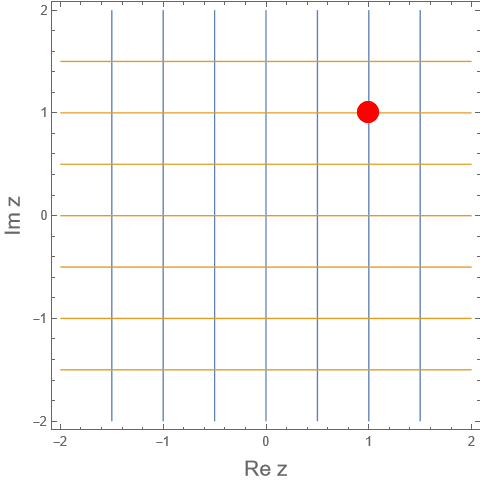
\includegraphics[width=\linewidth]{5_4.png}
		\caption{$f(z)=z$.}
		\label{fig:ej_5_4}
	\end{subfigure}
	\begin{subfigure}{0.3\textwidth}
		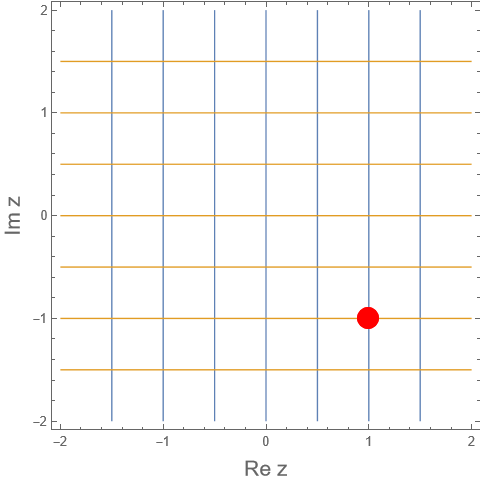
\includegraphics[width=\linewidth]{5_5.png}
		\caption{$f(z)=\overline{z}$.}
		\label{fig:ej_5_5}
	\end{subfigure}
	\caption{Comportamiento discreto de las funciones $f(z)=z$ y $f(z)=\overline{z}$}
	\label{fig:ej_5D}
\end{figure}
\end{Ejem} 



\begin{Ejem}
	Sea 
	\[
		f(z)= \left\{\begin{array}{ccl}
			\dfrac{(z)^5}{|z|^4}, &\mbox{ sí }& z\neq 0\\
			0,&\mbox{ sí }&z=0.
		\end{array} \right. 
	\] 
	 Sí $z=x+iy$, tenemos que $$z^5=x^5+5ix^4y-10x^3y^2-10ix^2y^3+5xy^4+iy^5,$$ así como $$|z|^4=x^4+2 x^2 y^2+y^4.$$
	 Entonces $$u(x,y)=\dfrac{x^5 - 10 x^3 y^2  + 5 x y^4 }{x^4 + 2 x^2 y^2 + y^4},$$  $$v(x,y)=\dfrac{ 5  x^4 y  - 10  x^2 y^3 +  y^5}{x^4 + 2 x^2 y^2 + y^4}.$$Luego
	\[
		\begin{array}{ccl}
			u_x(0,0)&=&\ds\lim_{x\rightarrow 0}\dfrac{u(x,0)-u(0,0)}{x}\\\\
			&=&\ds\lim_{x\rightarrow 0}\dfrac{\frac{x^5}{x^4}}{x}\\\\
			&=&\ds\lim_{x\rightarrow 0}\dfrac{x^5}{x^5}\\\\
			&=&1,\\
			v_y(0,0)&=&\ds\lim_{y\rightarrow 0}\dfrac{v(0,y)-v(0,0)}{y}\\
			&=&\ds\lim_{y\rightarrow 0}\dfrac{y^5}{y^5}\\
			&=&1,\\
			u_y(0,0)&=&\ds\lim_{y\rightarrow 0}\dfrac{u(0,y)-u(0,0)}{y}\\\\
			&=&\ds\lim_{y\rightarrow 0}\dfrac{\dfrac{0}{y^4}}{y}\\\\
			&=&\ds\lim_{y\rightarrow 0}\dfrac{0}{y}\\\\
			&=&0,\\
			v_x(0,0)&=&\ds\lim_{x\rightarrow 0}\dfrac{v(x,0)-v(0,0)}{x}\\\\
			&=&\ds\lim_{x\rightarrow 0}\dfrac{\dfrac{0}{x^4}}{x}\\\\
			&=&\ds\lim_{x\rightarrow 0}\dfrac{0}{x}\\
			&=&0.
		\end{array}
	\]
	Luego $f$ satisface las ecuaciones de Cauchy-Riemann en $z=0$.\\
	Por otro lado, tomemos $z=te^{i\theta}$ con $\theta\in \R$ fijo y $t>0$  tal que $t\rightarrow0^{+}$, entonces
	\[
		\begin{array}{ccl}
			f'(z)&=&\ds\lim_{z\rightarrow0}\ds\dfrac{f(z)-f(0)}{z}\\\\
			&=&\ds\lim_{t\rightarrow0}\dfrac{f(te^{i\theta})}{te^{i\theta}}
		\end{array}
	\]
	Desarrollando $f(te^{i\theta})$, 
	\[
	\begin{array}{ccl}
		f(te^{i\theta})&=&\dfrac{(te^{i\theta})^5}{|te^{i\theta}|^4}\\\\
		&=&\dfrac{t^5e^{5i\theta}}{|t|^4|e^{i\theta}|^4}\\\\
		&=&\dfrac{t^5e^{5i\theta}}{t^4 |\cos\theta+i\sen \theta|^4}\\\\
		&=&te^{5i\theta}
	\end{array}
	\]
	Entonces, 
	$$f'(z)=\ds\lim_{t\rightarrow0}=\dfrac{te^{5i\theta}}{te^{i\theta}}=e^{4i\theta}$$
	
	%&=&\ds\lim_{t\rightarrow0}\dfrac{(te^{i\theta})^5/|te^{i\theta}|^4}{te^{i\theta}}\\\\
	%&=&\ds\lim_{t\rightarrow0}\dfrac{t^5e^{i4\theta}}{t^5}\\\\
	Por otra parte,  $u_x(0,0)+iv_x(0,0)=1$, por lo tanto $f'(0)$ no puede existir. \\
	Usando \textbf{Mathematica}
	\begin{mmaCell}{Input}
		ComplexPlot[(z)^5/((Abs[z])^4), \{z, -2 - 2 I, 2 + 2 I\}]
	\end{mmaCell}
	
	\begin{mmaCell}{Input}
		ComplexPlot3D[(z)^5/((Abs[z])^4), \{z, -2 - 2 I, 2 + 2 I\}]
	\end{mmaCell}
	
	\begin{mmaCell}{Input}
		ComplexContourPlot[\{Re[(z)^5/((Abs[z])^4)],\\Im[(z)^5/((Abs[z])^4)]\}, \{z, 2\},\\PlotLegends -> "Expressions"]
	\end{mmaCell}
	obtenemos las graficas mostradas en la figura \ref{fig:ej_6}.\\	
	\begin{figure}[htbp!]
		\centering
		\begin{subfigure}{0.2\textwidth}
			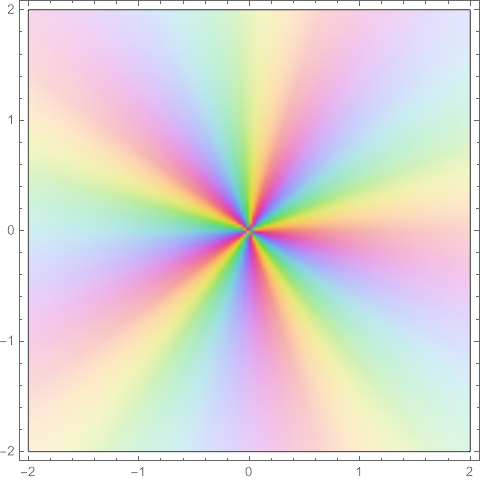
\includegraphics[width=\linewidth]{6_1.png}
			\caption{ComplexPlot.}
			\label{fig:ej_6_1}
		\end{subfigure}
		\begin{subfigure}{0.3\textwidth}
			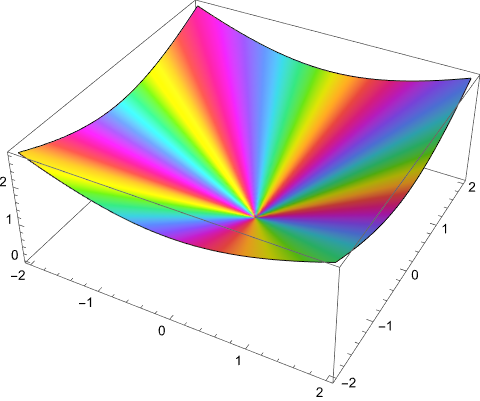
\includegraphics[width=\linewidth]{6_2.png}
			\caption{ComplexPlot3D.}
			\label{fig:ej_6_2}
		\end{subfigure}
		\begin{subfigure}{0.3\textwidth}
			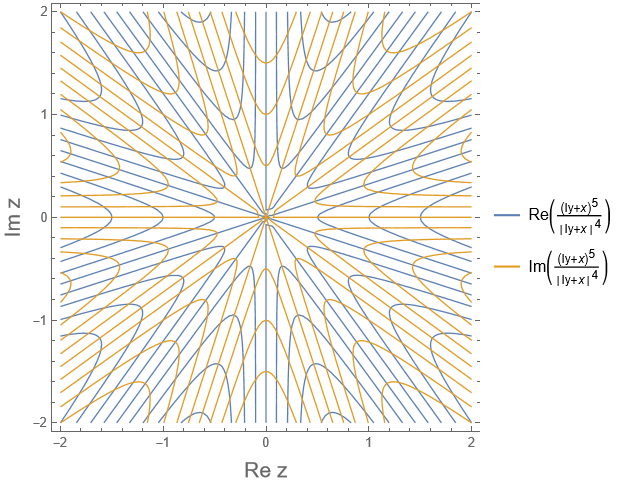
\includegraphics[width=\linewidth]{6_3.png}
			\caption{ComplexContourPlot.}
			\label{fig:ej_6_3}
		\end{subfigure}
		\caption{Diferentes representaciones gráficas de la función $f(z)=\frac{(z)^5}{|z|^4}$}
		\label{fig:ej_6}
	\end{figure}
	
	En las figuras \ref{fig:ej_6_1} y \ref{fig:ej_6_2} podemos ver que la función $f(z)=\frac{(z)^5}{|z|^4}$ tiene un cero de orden 5 en $z=0$, mientras que en la figura \ref{fig:ej_6_3} vemos que la se mapean las componentes reales e imaginarias.
\end{Ejem} 

Hay algunas consecuencias básicas de las ecuaciones de Cauchy-Riemann, las cuales se derivan fácilmente y que tienen consecuencias muy importantes, especialmente en el desarrollo de aplicaciones en matemáticas aplicadas.\\
Considere las curvas $u(x,y)=\mbox{cte}$, $v(x,y)=\mbox{cte}$. El gradiente, $\operatorname{grad } u$, es
\[
	\mbox{grad } u=\left(\begin{array}{c}
		\dpartial{u}{x}\\\\
		\dpartial{u}{y}
	\end{array}\right).
\]
Similarmente para $v$. Las ecuaciones de Cauchy-Riemann implican que 
$$\left(\dpartial{u}{x}\right)^2+\left(\dpartial{u}{y}\right)^2=\left(\dpartial{v}{x}\right)^2+\left(\dpartial{v}{x}\right)^2,$$
y $$\dpartial{u}{x}\dpartial{v}{x}+\dpartial{u}{y}\dpartial{v}{y}=0.$$

\begin{teor}\label{Teor8.5silv}
	Si $f(z)$ es analítica en un dominio G, entonces $f(z)$ tiene derivadas de todos los ordenes en $G$, más aún toda derivada $$f^{n}(z)=\dfrac{d^n f(z)}{dz^n},$$ es analítica en $G$ para toda $n=0,1,2,\ldots$.\\
	Una demostración de este teorema puede encontrarla en \cite{silverman}, más precisamente el Teorema 8.5. 
\end{teor}
Ahora, usando el Teorema \ref{Teor8.5silv}, podemos derivar nuevamente y también intercambiar el orden de diferenciación, además de usar las ecuaciones de Cauchy-Riemann para obtener que
$$\dpartial{^2 u}{x^2}=\dfrac{\partial}{\partial x}\left(\dpartial{u}{x}\right)=\dfrac{\partial}{\partial x}\left(\dpartial{v}{x}\right)=\dfrac{\partial}{\partial y}\left(\dpartial{v}{x}\right)=-\dfrac{\partial}{\partial y}\left(\dpartial{u}{y}\right)=-\dpartial{^2u}{y^2},$$
luego
$$\dpartial{^2 u}{x^2}+\dpartial{^2u}{y^2}=0,$$
entonces $u$ satisface la ecuación de Laplace, en este caso diremos que la función es armónica. Similarmente para $v$.

\section{El Teorema de Ahlfors-Struble}
 Sean $z = x + iy$ y $f(z) = u(x, y)+iv(x, y)$. Entonces dada una función $u(x, y)$, a menudo surge la pregunta de cómo encontrar la función $v(x,y)$ correspondiente y, por tanto, el mapeo  $f(z)$. En la mayoría de las veces el problema se soluciona resolviendo las ecuaciones de Cauchy-Riemann. Tenga en cuenta que un paso preliminar y muy sensato es comprobar que $u(x,y)$  satisface la ecuación de Laplace, esto se ilustra en el siguiente ejemplo.
 \begin{Ejem}\label{EjCR}
 	Sea $u(x,y)=x^2-y^2$, encuentre $v(x,y)$ tal que $f(z)=u(x,y)+iv(x,y)$ sea complejo diferenciable.
 	\solu
 	\noindent En primer lugar, planteamos nuestro sistema de ecuaciones de Cauchy-Riemann
 	\[
 		\begin{array}{c}
 			\dpartial{u}{x}=\dpartial{v}{y}=2x,\\\\
 			\dpartial{u}{y}=-\dpartial{v}{x}=-2y,
 		\end{array}
 	\]
 	luego integramos las parciales de $v$ y obtenemos
 	\[
 		\begin{array}{c}
 			v(x,y)=2xy+g(x),\\
 			v(x,y)=2yx+h(y),
 		\end{array}
 	\]
 	donde $g,h$ son funciones arbitrarias. Igualando las dos expresiones anteriores, se tiene que $g(x)=h(y)$, es decir, $g$ y $h$ deben de ser constantes. Luego $v=2xy+c$ para alguna constante $c$, por tanto 
 	$$f(z)=x^2-y^2+2ixy+ic=(x+iy)^2+ic=z^2+ic.$$\endproof
 \end{Ejem}
Este ejemplo resulta ser muy simple, pero en ocasiones podemos encontrarnos algunos en los cuales la obtención  de $v$ y
por ende de $f$ no son tan sencillos, por ejemplo  la función 
$$u(x,y)=e^{\dfrac{x}{x^2+y^2}}\cos\left(\dfrac{y}{x^2+y^{2}}\right).$$
Este ejemplo lo estudiaremos más adelante utilizando un Teorema que en seguida se enunciara.\\
El Teorema de Ahlfors-Struble nos proporciona un método donde podemos encontrar $f$ a partir de $u$ (o a partir de $v$) de una manera puramente algebraica. El teorema se presenta en dos versiones, la primera de ellas es cuando $f(z)$ es una función complejo diferenciable en una vecindad en el origen y la segunda,  cuando $f(z)$ es una función complejo diferenciable en una vecindad de $a\neq 0$.\\
\noindent Se tiene la siguiente definición
\begin{defi}
	Sea $u:\R^2\rightarrow\R$ una función real, por una extensión natural de $u$ nos referiremos a un función $u_{ex}:\C^2\rightarrow\C$ que se obtiene al sustituir $x,y\in\R$ en $u$ por $w_1,w_2\in\C$.
\end{defi}
\noindent Si $f(z)$ es una función diferenciable en una vecindad en el origen y $\tilde{u}:\C^2\rightarrow\C$ es una función dada por
\begin{equation}\label{AS1}
	\title{u}(w_1,w_2)=\dfrac{1}{2}[f(w_+i_w2)+\hat{f}(w_1-iw_2)],
\end{equation}
en donde  $\hat{f}$ es la reflexión, $\hat{f}:\C\rightarrow\C$ dada por $\hat{f}(z)=\overline{f(\overline{z})}$.\\
\noindent Note que, si  hacemos el cambio de variable 
\begin{equation}\label{AS2}
	w_1=\dfrac{z}{2},\;\;\;w_2=\dfrac{z}{2i},
\end{equation}
donde $z\in\C$, obtenemos 
\begin{equation}\label{AS3}
	\tilde{u}\left(\dfrac{z}{2},\dfrac{z}{2i}\right)=\dfrac{1}{2}[f(z)+\hat{f}(0)]=\dfrac{1}{2}[f(z)+\overline{f(0)}]
\end{equation}
Observemos que si $w_1=x$ y $w_2=y$ con $x,y\in\R$, entonces 
\[
	\begin{array}{ccl}
		\tilde{u}(x,y)&=&\dfrac{1}{2}[f(x+iy)+\hat{f}(x-iy)]\\\\
		&=&\dfrac{1}{2}[f(x+iy)+\overline{f(x+iy)}]\\
		&=&u(x,y),
	\end{array}
\]
ya que para cualquier $z\in\C$ se verifica que $z+\overline{z}=2\operatorname{Re}(z)$. Del análisis anterior, se tiene que $\tilde{u}$ es extensión natural de $\C^2$ de la función real $u(x,y)$. Entonces
\[
	\begin{array}{ccl}
		u\left(\dfrac{z}{2},\dfrac{z}{2i}\right)&=&u_{ex}\left(\dfrac{z}{2},\dfrac{z}{2i}\right)\\\\
		&=&\tilde{u}\left(\dfrac{z}{2},\dfrac{z}{2i}\right)\\\\
		&=&\dfrac{1}{2}[f(z)+\overline{f(0)}]
	\end{array}
\]
El razonamiento anterior, es un esbozo de la demostración del siguiente teorema.

\begin{teor}[Ahlfors-Struble para vecindades en torno al origen]\label{TAS1}
	Sea $f(z)$ diferenciable en una vecindad del origen, con parte real $u(x, y)$ y parte imaginaria $v(x, y)$, donde 
	$z = x + iy$. Entonces, se tiene
	\[
		\begin{array}{ccl}
			f(z)&=&2u\hspace{-0.1cm}\left(\dfrac{z}{2},\dfrac{z}{2i}\right)-\overline{f(0)}\\\\
			&=&2iv\hspace{-0.1cm}\left(\dfrac{z}{2},\dfrac{z}{2i}\right)+\overline{f(0)},
		\end{array}
	\]
	donde $\overline{f(0)}$ es el conjugado de $f(0)$.
\end{teor}
Consideremos nuevamente el ejemplo \ref{EjCR}, pero ahora lo resolveremos usando el Teorema \ref{TAS1}.
\begin{Ejem}	
	Sea $u(x,y)=x^2-y^2$, encuentre  $f(z)$ usando el Teorema \ref{TAS1}.
	\solu
	\noindent Note que $u(0, 0) = 0$, por lo que $f(0) = i\beta$ para alguna $\beta\in\R$. Aplicando el Teorema \ref{TAS1}
	\[
		\begin{array}{ccl}
			f(z)&=&2u\left(\dfrac{z}{2},\dfrac{z}{2i}\right)-\overline{f(0)}\\
			&=&2\left(\left(\dfrac{z}{2}\right)^2-\left(\dfrac{z}{2i}\right)^2\right)-\overline{f(0)}\\
			&=&2\left(\dfrac{z^2}{4}+\dfrac{z^2}{4}\right)-\overline{i\beta}\\
			&=&z^2+i\beta.
		\end{array}
	\]
	Con  $\beta=0$. 
	\begin{mmaCell}{Input}
		ComplexPlot[z^2, \{z, -2 - 2 I, 2 + 2 I\}]
	\end{mmaCell}
	
	\begin{mmaCell}[moregraphics={moreig={scale=.25}}]{Output}
		\mmaFrac{ \mmaGraphics{8_1.png}}{}
	\end{mmaCell}
 Notemos que en imagen obtenida se tiene que patrón de los colores se repite dos veces alrededor del $0$, esto se debe a que en este punto la función $f(z)=z^2$ tiene un cero de multiplicidad 2.\endproof
\end{Ejem}

\begin{Ejem}	
	Sea $u(x,y)=e^{x} \cos(y)$, encuentre $v(x,y)$ tal que $f(z)=u(x,y)+iv(x,y)$ sea complejo diferenciable.
	\solu
	\noindent Vemos que $u(0,0)=1$, luego $f(0)=1+i\beta$ para  alguna $\beta\in\R$. Recordemos que 
	$$\cos p=\dfrac{1}{2}(e^{ip}+e^{-ip}).$$
	Entonces 
	\[
		\begin{array}{ccl}
			f(z)&=&2e^{\frac{z}{2}}\cos\left(\dfrac{z}{2i}\right)-\overline{1+i\beta}\\
			&=&e^{\frac{z}{2}}\left[e^{i\frac{z}{2i}}+e^{-i\frac{z}{2i}} \right]-1+i\beta\\
			&=&e^{z}+i\beta.
		\end{array}
	\]
	Con $\beta=1$
	
	\begin{mmaCell}{Input}
		ComplexPlot[Exp[z] + I,\{z, -10 - 10 I, 10 + 10 I\},\\PlotRange -> Automatic]
	\end{mmaCell}
	
	\begin{mmaCell}[moregraphics={moreig={scale=.25}}]{Output}
		\mmaFrac{ \mmaGraphics{9_1.png}}{}
	\end{mmaCell}
Usando el comando \textbf{Solve} podemos encontrar las soluciones  de la función $f(z)$,
\begin{mmaCell}{Input}
	 Solve[Exp[z] == -I, z]
\end{mmaCell}
de lo anterior obtenemos que las soluciones son $$\left\{z\mid -\dfrac{i\pi}{2} +2 i \pi  k\text{ si }k\in \Z\right\}.$$
Usando un bucle \textbf{For}, obtenemos numéricamente las 3 soluciones que se muestran en la imagen.
\begin{mmaCell}{Input}
	 For[i = -1, i < 2, i++, Print[-0.5*(I*Pi) + 2*I*Pi*i]]
\end{mmaCell}
los cuales resultan ser $-7.85398 i,  -1.5708 i$ y $4.71239i$ para $k=-1,0,1$ respectivamente.\endproof

\end{Ejem}


\begin{teor}[Ahlfors-Struble para vecindades en torno a puntos distintos al origen]\label{TAS2}
	Sea $f(z)$ complejo diferenciable en una vecindad del punto $a$, con parte real $u(x, y)$ y parte imaginaria $v(x, y)$, donde 
	$z = x + iy$. Entonces extendiendo  $u$ (o $v$) a $\C^2$ se tiene
	\[
	\begin{array}{ccl}
		f(z)&=&2u\hspace{-0.1cm}\left(\dfrac{z+\bar{a}}{2},\dfrac{z-\bar{a}}{2i}\right)-\overline{f(a)}\\
		&=&2iv\hspace{-0.1cm}\left(\dfrac{z+\bar{a}}{2},\dfrac{z-\bar{a}}{2i}\right)+\overline{f(a)},
	\end{array}
	\]
	donde $\overline{f(a)}$ es el conjugado de $f(a)$.\\
		La demostración de este teorema se puede consultar en \cite{Shaw-A}, vea el Teorema 2.1.
\end{teor}


\begin{Ejem}[Una función con un polo simple en el origen]
	Sea $u(x,y)=\dfrac{x}{x^2+y^2}$, encuentre $f(z)$.
	\solu Note que 
	$$\left(\dfrac{z+\bar{a}}{2}\right)^{2}+\left(\dfrac{z-\bar{a}}{2i}\right)^2=\dfrac{(z+\overline{a})^2-(z-\overline{a})^2}{4}=\dfrac{4z\overline{a}}{4}=z\overline{a}.$$
	Usando el Teorema \ref{TAS2}
	\[
		\begin{array}{ccl}
			f(z)&=&2u\left(\dfrac{z+\bar{a}}{2},\dfrac{z-\bar{a}}{2i}\right)-\overline{f(a)}\\\\
			&=&2\left(\dfrac{\dfrac{z+\bar{a}}{2}}{\left(\dfrac{z+\bar{a}}{2}\right)^{2}+\left(\dfrac{z-\bar{a}}{2i}\right)^2}\right)-\overline{f(a)}\\\\
			&=&2\dfrac{z+\bar{a}}{2}\dfrac{1}{z\bar{a}}-\overline{f(a)}\\\\
			&=&\dfrac{1}{z}+\dfrac{1}{\overline{a}}-\overline{f(a)}.
		\end{array}
	\]
	Vemos que en $z = a$ se tiene la relación $f(a)+\overline{f(a)}=\frac{1}{a}+\frac{1}{\overline{a}}$, es decir, tenemos  que la parte real de $f(a)$ es la parte real de $\frac{1}{\overline{a}}$ , entonces se infiere que
	$$f(z)=\dfrac{1}{z}+i\beta,$$
	con $\beta\in\R$.\\Tomemos $\beta=0$,
	\begin{mmaCell}{Input}
		ComplexPlot[1/z, \{z, -10 - 10 I, 10 + 10 I\},\\PlotRange -> All]
	\end{mmaCell}
	
	\begin{mmaCell}[moregraphics={moreig={scale=.50}}]{Output}
		\mmaFrac{ \mmaGraphics{11_1_1.png}}{}
	\end{mmaCell}
En la imagen anterior, podemos observar que el giro de los colores se invierte, es decir, siguen el giro de las manecillas del reloj. El comportamiento se debe a que esta función tiene un polo simple en el origen. \endproof
\end{Ejem}
\begin{teor}[Teorema Grande de Picard]\label{GTP}
	Sea $a$ una singularidad esencial de $f$ en alguna vecindad agujerada. Entonces para cada vecindad agujerada de $a$, $f(z)$ asume todos los números complejos, con una posible excepción, un número infinito de veces.
	La prueba de este teorema se puede consultar en \cite{Conway}, vea el Teorema 4.2.
\end{teor}
\begin{Ejem}[Una función con una singularidad esencial en el origen]\label{ejem9}
	Sea $$u(x,y)=e^{\dfrac{x}{x^2+y^2}}\cos\left(\dfrac{y}{x^2+y^2}\right),$$  encuentre $f(z)$.
	\solu Tenemos que si $x\rightarrow\frac{z+\overline{a}}{2}$, $y\rightarrow\frac{z-\overline{a}}{2i}$
	\[
		\begin{array}{ccl}
			\dfrac{x}{x^2+y^2}&=&\dfrac{\dfrac{z+\overline{a}}{2}}{\left(\dfrac{z+\overline{a}}{2}\right)^2+\left(\dfrac{z-\overline{a}}{2i}\right)^2}\\
			&=&\dfrac{\dfrac{z+\overline{a}}{2}}{\dfrac{(z+\overline{a})^2-(z-\overline{a})^2}{4}}\\
			&=&\dfrac{\dfrac{z+\overline{a}}{2}}{\dfrac{4\overline{a}z}{4}}\\
			&=&\dfrac{z+\overline{a}}{2z\overline{a}},\\
				\end{array}
			\]
			
			\[
			\begin{array}{ccl}
			\dfrac{y}{x^2+y^2}&=&\dfrac{\dfrac{z-\overline{a}}{2i}}{\left(\dfrac{z+\overline{a}}{2}\right)^2+\left(\dfrac{z-\overline{a}}{2i}\right)^2}\\\\
			&=&\dfrac{\dfrac{z-\overline{a}}{2i}}{\dfrac{(z+\overline{a})^2-(z-\overline{a})^2}{4}}\\\\
			&=&-\dfrac{\dfrac{z-\overline{a}}{2i}}{\dfrac{4\overline{a}z}{4}}\\\\
			&=&-\dfrac{z-\overline{a}}{2iz\overline{a}},
		\end{array}
	\]
	luego
	\[
		\begin{array}{ccl}
			f(z)&=&2\exp\left({\dfrac{z+\overline{a}}{2z\overline{a}}}\right)\cos\left(\dfrac{z-\overline{a}}{2iz\overline{a}}  \right)-\overline{f(a)}\\\\
			&=&2\exp\left({\dfrac{1}{2\overline{a}}+\dfrac{1}{2z}}\right)\cos\left(\dfrac{1}{2i\overline{a}}-\dfrac{1}{2iz}\right)-\overline{f(a)}.
				\end{array}
			\]
			Recordemos que el coseno se puede escribir en términos de la exponencial:
			$$\cos\alpha=\dfrac{1}{2}\left(e^{i\alpha}+e^{-i\alpha}\right).$$
			Entonces
			$$2\cos\left(\dfrac{1}{2i\overline{a}}-\dfrac{1}{2iz}\right)=\exp\left(\dfrac{1}{2\overline{a}}-\dfrac{1}{2z}\right)+\exp\left(-\dfrac{1}{2\overline{a}}+\dfrac{1}{2z}\right)$$
			por lo que 
			\[
			\begin{array}{ccl}
			f(z)&=&\exp\left({\dfrac{1}{2\overline{a}}+\dfrac{1}{2z}}\right)\left(\exp\left(\dfrac{1}{2\overline{a}}-\dfrac{1}{2z}\right)+\exp\left(-\dfrac{1}{2\overline{a}}+\dfrac{1}{2z}\right)\right)\\\\
			&=&\exp\left({\dfrac{1}{z}}\right)+\exp\left({\dfrac{1}{\overline{a}}}\right)-\overline{f(a)},\\\\
		\end{array}
	\]
	Si $z=a$, entonces $$f(a)+\overline{f(a)}=\exp\left({\dfrac{1}{z}}\right)+\exp\left({\dfrac{1}{\overline{a}}}\right),$$ es decir, $$2\operatorname{Re} (f(a))=2\operatorname{Re }\left(\exp\left(\dfrac{1}{a}\right)\right)\implies \operatorname{Re }(f(a))=\operatorname{Re }\left(\exp\left(\dfrac{1}{a}\right)\right).$$
	Dado que $f(a),\exp\left(\dfrac{1}{a}\right)\in \C$, entonces, los podemos reescribir como 
	$$f(a)=\alpha_1+\beta_1 i,$$
	$$\exp\left(\dfrac{1}{a}\right)=\alpha_2+\beta_2 i,$$
	y por el análisis previo se debe de tener que $\alpha_1=\alpha_2$, para simplificar $\alpha=\alpha_1=\alpha_2$, entonces 
	\[
	\begin{array}{ccl}
		f(z)&=&\exp\left({\dfrac{1}{z}}\right)+\exp\left({\dfrac{1}{\overline{a}}}\right)-\overline{f(a)}\\\\
		&=&\exp\left({\dfrac{1}{z}}\right)+\overline{\exp\left({\dfrac{1}{a}}\right)}-\overline{f(a)}\\\\
		&=&\exp\left(\dfrac{1}{z}\right)+\overline{\alpha_2+\beta_2 i}+\overline{\alpha_1+\beta_1 i}\\\\
		&=&\exp\left(\dfrac{1}{z}\right)+\overline{\alpha+\beta_2 i}+\overline{\alpha+\beta_1 i}\\\\
		&=&\exp\left(\dfrac{1}{z}\right)+\alpha-\beta_2 i-\alpha+\beta_1 i\\\\
		&=&\exp\left(\dfrac{1}{z}\right)+(\beta_1-\beta_2)i,
	\end{array}
	\]
	Si $\beta=\beta_1-\beta_2$, entonces $$\exp\left({\dfrac{1}{z}}\right)+\beta i$$
	donde  $\beta\in \R$.\\
	Para simplificar, si tomamos $\beta=0$,  entonces $f(z)=e^{\frac{1}{z}}$.\begin{mmaCell}{Input}
		ComplexPlot[Exp[1/z], \{z, -1 - 1 I, 1 + 1 I\},\\PlotRange -> Automatic,ColorFunction -> "CyclicLogAbs"]
	\end{mmaCell}
	
	\begin{mmaCell}[moregraphics={moreig={scale=.25}}]{Output}
		\mmaFrac{ \mmaGraphics{11_2.png}}{}
	\end{mmaCell}
La función anterior es bastante interesante, ya que al representarla con colores podemos ver que no hay ningún punto en el cual los colores giren en torno a él, pero justo en el punto $z=0$, vemos como los colores se van alternando infinitamente hasta acercarse  al $0$, este comportamiento de los colores se da cuando se tiene una singularidad esencial.\\
Visualmente, lo que podemos ver en la figura, es que la función $e^{\frac{1}{z}}$ toma todos los valores complejos, excepto el $0$, en cualquier vecindad del origen; es decir, esta función satisface el Teorema \ref{GTP}.\endproof
\end{Ejem}


\begin{Ejem}[Una función con un punto de ramificación en el origen]
	Sea $$u(x,y)=\ln(\sqrt{x^2+y^2}),$$  encuentre $f(z)$.
	\solu
	Se tiene que $$u(x,y)=\ln(\sqrt{x^2+y^2})=\dfrac{1}{2}\ln(x^2+y^2),$$
	entonces 
	\[
		\begin{array}{ccl}
			f(z)&=&2\dfrac{1}{2}\ln(z\overline{a})-\overline{f(a)}\\
			&=&\ln(z)+\ln(\overline{a})-\overline{f(a)}\\
			&=&\ln(z)+i\beta,
		\end{array}
	\]
	donde $\beta\in \R$ y se obtiene siguiendo el razonamiento seguido en el Ejemplo \ref{ejem9}.\\
	Tomando $\beta=0$, entonces $f(z)=e^{\frac{1}{z}}$.
	\begin{mmaCell}{Input}
		ComplexPlot[Log[z], \{z, -2 - 2 I, 2 + 2 I\},\\PlotRange -> Automatic,ColorFunction -> "CyclicLogAbs"]
	\end{mmaCell}
	
	\begin{mmaCell}[moregraphics={moreig={scale=.25}}]{Output}
		\mmaFrac{ \mmaGraphics{12_1.png}}{}
	\end{mmaCell}
\end{Ejem}
Notemos que, en la imagen anterior hay un punto en donde todos los colores se juntan y además la secuencia de colores va en sentido antihorario (azul, rojo, verde), es decir, la función $f(z)$ se anula en dicho punto, el cual resulta ser en el punto $z=1$. Además podemos observar como a la izquierda se juntan algunos colores en una línea  y esto ocurre en torno al cero, podemos ver que el logaritmo presenta ''problemas'' de continuidad, lo anterior está relacionado con las ramas del logaritmo y el punto $z=0$ es un punto de ramificación del logaritmo.\endproof

\subsection{Implementación del algoritmo en Mathematica }
Como expusimos antes, la formula  del Teorema \ref{TAS1} nos permite encontrar $f(z)$ a partir de $u$ o $v$ de forma algebraica. Es por ello que nos proponemos a realizar una implementación del Teorema \ref{TAS1} usando Mathematica, desde luego, utilizaremos esta implementación para realizar una comprobación de los ejemplos presentados anteriormente.\\
\noindent En nuestra implementación usaremos la función \textbf{ComplexExpand} con la opción \textbf{TargetFunctions -> \{Re, Im\}} para obtener la forma correcta de la función en términos de la variable compleja $z$.\\
\noindent Antes de realizar la implementación, expliquemos las funciones mencionadas en el párrafo anterior. En el caso de la función \textbf{ComplexExpand}, nos podemos dar una idea (por el nombre) de lo que realiza esta. Para usar esta función, debemos de pasar por parámetro obligatorio una expresión (\textit{expr}) y opcionalmente una lista de variables $\{x_1,x_2,\ldots,x_n\}$.  Si solo pasamos una expresión \textit{expr}, \textbf{ComplexExpand} solo   expande \textit{expr} asumiendo que todas las variables son reales.En cambio, si le pasamos una lista de variables, \textbf{ComplexExpand} expande \textit{expr} asumiendo que las variables que coinciden con cualquiera de $x_i$ son complejas. SE presentan algunos ejemplos a continuación.

\begin{mmaCell}{Input}
 	 ComplexExpand[Sin[x + I y]]
\end{mmaCell}

\begin{mmaCell}{Output}
	 Cosh[y] Sin[x] + I Cos[x] Sinh[y]
\end{mmaCell}

\begin{mmaCell}{Input}
	 ComplexExpand[Sin[x] Exp[y], {x, y}]
\end{mmaCell}

\begin{mmaCell}{Output}
	 E\^Re[y] Cos[Im[y]] Cosh[Im[x]] Sin[Re[x]] - E\^Re[y] Cos[Re[x]]\\Sin[Im[y]] Sinh[Im[x]] + I (E\^Re[y] Cosh[Im[x]] Sin[Im[y]] \\Sin[Re[x]] + E\^Re[y] Cos[Im[y]] Cos[Re[x]] Sinh[Im[x]])
\end{mmaCell}

La opción \textbf{TargetFunctions -> \{Re, Im\}}, de la función en cuestión, nos da la respuesta en términos de \textbf{Re[z]} y \textbf{Im[z]}

\begin{mmaCell}{Input}
	 ComplexExpand[Tan[z], {z}, TargetFunctions -> {Re, Im}]
\end{mmaCell}

\begin{mmaCell}{Output}
	 \mmaFrac{Sin[2 Re[z]]}{(Cosh[2 Im[z]] + Cos[2 Re[z]])} +\\ \mmaFrac{(I Sinh[2 Im[z]])}{(Cosh[2 Im[z]] + Cos[2 Re[z]])}
\end{mmaCell}
Con lo anterior ya explicado, podemos proceder a la implementación. En esta implementación, desarrollaremos una función que tomara tres parámetros, $expr$, $a$, y una una lista de tres elementos $\{xsym_, ysym_, zsym_ \}$, esta función la llamaremos \textbf{AhlforsStruble1}

\begin{mmaCell}{Input}
	 AhlforsStruble1[expr_, a_, {xsym_, ysym_, zsym_ }] := Module[\\ \{abar = Conjugate[a], exprf\},\\ exprf = ComplexExpand[expr, TargetFunctions -> \{Re, Im\}];\\ func = 2*exprf /. \{xsym -> (zsym + abar)/2, ysym ->\\ (zsym - abar)/(2*I)\};\\ basecorr =  - exprf /. {xsym -> Re[a], ysym -> Im[a]};\\ FullSimplify[func + basecorr + I*\(\pmb{\beta}\)]]
\end{mmaCell}
\noindent Para probar esta función, crearemos una lista de expresiones, estas expresiones serán las funciones  $u$ de los ejemplos anteriores.

\begin{mmaCell}{Input}
	 ConjuntoTestU = \{x^2 - y^2,\\ Exp[x] Cos[y],\\ x/(x^2 + y^2),\\ Exp[x/(x^2 + y^2)] Cos[y/(x^2 + y^2)],\\ Log[Sqrt[x^2 + y^2]]\};
\end{mmaCell}
Usando la función \textbf{Map} de Mathematica y la lista anterior
\begin{mmaCell}{Input}
	  Map[AhlforsStruble1[#, 0.0, {x, y, z}] &, ConjuntoTestU]
\end{mmaCell}
\begin{mmaCell}{Output}
	 \{z^2 + I \(\pmb{\beta}\),\\ E^z + I\(\pmb{\beta}\),\\ Indeterminate,\\ Indeterminate,\\ Indeterminate\}
\end{mmaCell}
\noindent Como podemos ver en el resultado, nuestra implementación arroja un valor indeterminado, esto se debe a que falla cuando el origen no es un punto en el que las funciones estén definidas, sin embargo, si cambiamos el punto $a$, por ejemplo por $a=1$, entonces nuestra implementación funciona sin problemas.

\begin{mmaCell}{Input}
	 Map[AhlforsStruble1[#, 1, {x, y, z}] &, ConjuntoTestU]
\end{mmaCell}
\begin{mmaCell}{Output}
	 \{z^2 + I \(\pmb{\beta}\),\\ E^z + I\(\pmb{\beta}\),\\ 1/z + I \(\pmb{\beta}\),\\ E^(1/z) + I \(\pmb{\beta}\),\\ I \(\pmb{\beta}\) + Log[z]\}
\end{mmaCell}
\noindent Podemos ver que, estos resultados son los mismos que obtuvimos anteriormente.





















 